% Avance 2 · Detección de celdas solares defectuosas en imágenes EL · PDI 2026-III
% Compilar con XeLaTeX desde esta carpeta:  latexmk -xelatex informe.tex
% Todas las figuras y cifras salen de los scripts del repo (ver la sección "Reproducir").
\documentclass[10pt,a4paper]{article}

\usepackage{fontspec}
\usepackage[spanish,es-noshorthands,es-nodecimaldot,es-tabla]{babel}
\usepackage[a4paper,top=2cm,bottom=1.9cm,left=2.2cm,right=2.2cm,headheight=14pt]{geometry}
\usepackage{amsmath,amssymb}
\usepackage{graphicx}
\usepackage{booktabs,array,tabularx,multirow}
\usepackage[table]{xcolor}
\usepackage[most]{tcolorbox}
\usepackage{fancyhdr}
\usepackage{enumitem}
\usepackage{caption}
\usepackage{float}
\usepackage{placeins}
\usepackage[hidelinks]{hyperref}

\graphicspath{{../../reports/figures/}{../comun/}}

\definecolor{ud}{RGB}{128,57,61}
\definecolor{udsoft}{RGB}{242,230,231}
\definecolor{tinta}{RGB}{50,50,50}
\definecolor{gris}{RGB}{120,120,120}
\definecolor{okc}{RGB}{27,140,96}

\captionsetup{font=small,labelfont={bf,color=ud},labelsep=period}
\setlist{itemsep=1pt,topsep=2pt}
\setlength{\parskip}{3pt}
\setlength{\intextsep}{6pt plus 2pt}
\captionsetup{skip=3pt}
\setlength{\parindent}{0pt}

\pagestyle{fancy}\fancyhf{}
\fancyhead[L]{\small\color{gris}Celdas solares defectuosas en imágenes EL}
\fancyhead[R]{\small\color{gris}Avance 2 · PDI 2026-III}
\fancyfoot[C]{\small\color{gris}\thepage}
\renewcommand{\headrulewidth}{0.3pt}

\newtcolorbox{decision}[1]{enhanced,breakable,colback=udsoft,colframe=ud,boxrule=0.6pt,arc=1pt,
  left=6pt,right=6pt,top=4pt,bottom=4pt,fonttitle=\bfseries\small,coltitle=white,title={#1}}
\newtcolorbox{ojo}[1]{enhanced,breakable,colback=white,colframe=ud,boxrule=0.6pt,arc=1pt,
  borderline west={3pt}{0pt}{ud},left=8pt,right=6pt,top=4pt,bottom=4pt,
  fontupper=\small,title={#1},fonttitle=\bfseries\small,coltitle=ud,colbacktitle=white,attach title to upper={\quad}}

\newcommand{\hecho}{{\color{okc}$\checkmark$}}
\newcommand{\cifra}[2]{\begin{minipage}[t]{0.235\textwidth}\centering{\color{ud}\fontsize{20}{22}\selectfont #1}\par\vspace{2pt}{\footnotesize #2}\end{minipage}}


\begin{document}

\begin{minipage}[c]{0.14\textwidth}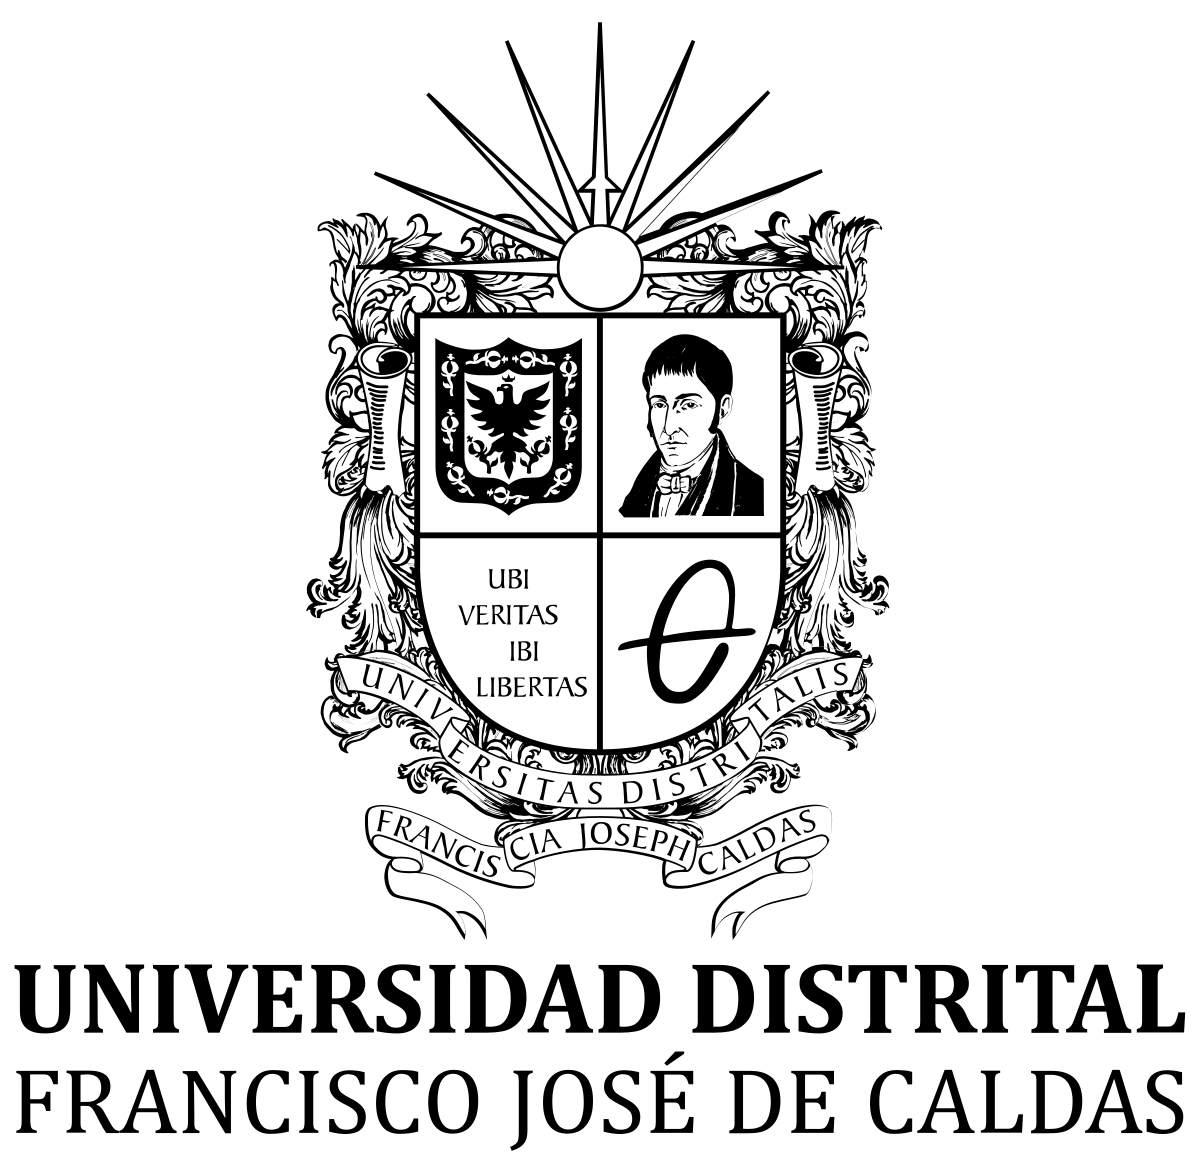
\includegraphics[width=\linewidth]{logo.png}\end{minipage}\hfill
\begin{minipage}[c]{0.83\textwidth}
  {\small\color{gris}Procesamiento Digital de Imágenes · Universidad Distrital Francisco José de Caldas}\par\vspace{3pt}
  {\LARGE\color{ud}Avance 2 · Quitar los busbars}\par\vspace{3pt}
  {\large Detección de celdas solares defectuosas en imágenes de electroluminiscencia}\par\vspace{4pt}
  {\small Joel Eduardo Reyes Barrios (20212005011) · Johan Sebastián Cáceres Rodríguez (20212005111) ·
   Hosman Javier Nieto Cruz (20212005117)}\par
  {\small\color{gris}Semana 2 del cronograma (16 – 22 de noviembre de 2026) · entregado el 25 de noviembre}
\end{minipage}
\vspace{6pt}
{\color{ud}\rule{\textwidth}{0.8pt}}

\section*{1 \quad Resumen}

Implementamos las dos formas de quitar los busbars, el notch en Fourier (A) y el cierre morfológico (B), y las comparamos en
validación con los criterios de imagen de la tabla 3. Antes hubo que rehacer la detección de los busbars, porque la de la semana 1
casi siempre añadía bandas falsas.

\vspace{4pt}
\noindent
\cifra{12 → 100\,\%}{celdas de validación con la rejilla detectada exacta: v1 frente a v2}\hfill
\cifra{0,9\,\%}{resto del busbar con el cierre (B). Con el notch: 5,9\,\% en toda la celda y 11,7\,\% solo en las filas}\hfill
\cifra{3\,\% \textit{vs.} 84\,\%}{contraste de una grieta a 45° que cruza un busbar: cierre frente a notch}\hfill
\cifra{−40\,\%}{respuesta de Sato que pierde una grieta vertical fina al quitar los dedos con $1\times3$}
\vspace{6pt}

\begin{decision}{Lo que decidimos y lo que falta decidir}
\begin{itemize}[leftmargin=12pt]
  \item \textbf{Detección v2} desde ahora: banda fina, de todo el ancho y con la geometría de la rejilla.
  \item \textbf{Notch o cierre: sin decidir.} B gana en los criterios 1, 2 y 4, que son de apoyo, pero borra las grietas inclinadas que
        cruzan un busbar. Decide el criterio 3 (AUC de la CNN), en la semana 3.
  \item \textbf{Proponemos no quitar los dedos.} Es un cambio frente a la propuesta (§4.3); lo confirmará la CNN.
\end{itemize}
\end{decision}

\section*{2 \quad Avance frente al cronograma}

\begin{table}[H]
\centering\small
\begin{tabularx}{\textwidth}{@{}c X >{\footnotesize}p{6.6cm}@{}}
\toprule
 & Actividad de la semana 2 (tabla 6 de la propuesta) & Dónde quedó \\
\midrule
\hecho & Detección de busbars por celda & \texttt{src/busbars.py}, \texttt{detectar()} \\
\hecho & Implementación del notch (A-global y A-filas) y del cierre (B) & \texttt{src/busbars.py} \\
\hecho & Comparación en validación con las métricas de imagen & \texttt{scripts/07\_comparar\_busbars.py} \\
\hecho & Dedos y revisión de las grietas verticales finas con Sato & \texttt{scripts/09\_grietas\_verticales.py} \\
\midrule
+ & Grietas sintéticas por ángulo y página interactiva & \texttt{entregas/avance\_2/web/} \\
\bottomrule
\end{tabularx}
\end{table}

Las actividades técnicas de la semana 2 están hechas, tres días después de su fecha. El criterio 3 es de la semana 3, como estaba previsto. Falta la
lectura cruzada del equipo y el ensayo.

\section*{3 \quad Métodos}

\begin{figure}[H]
\centering
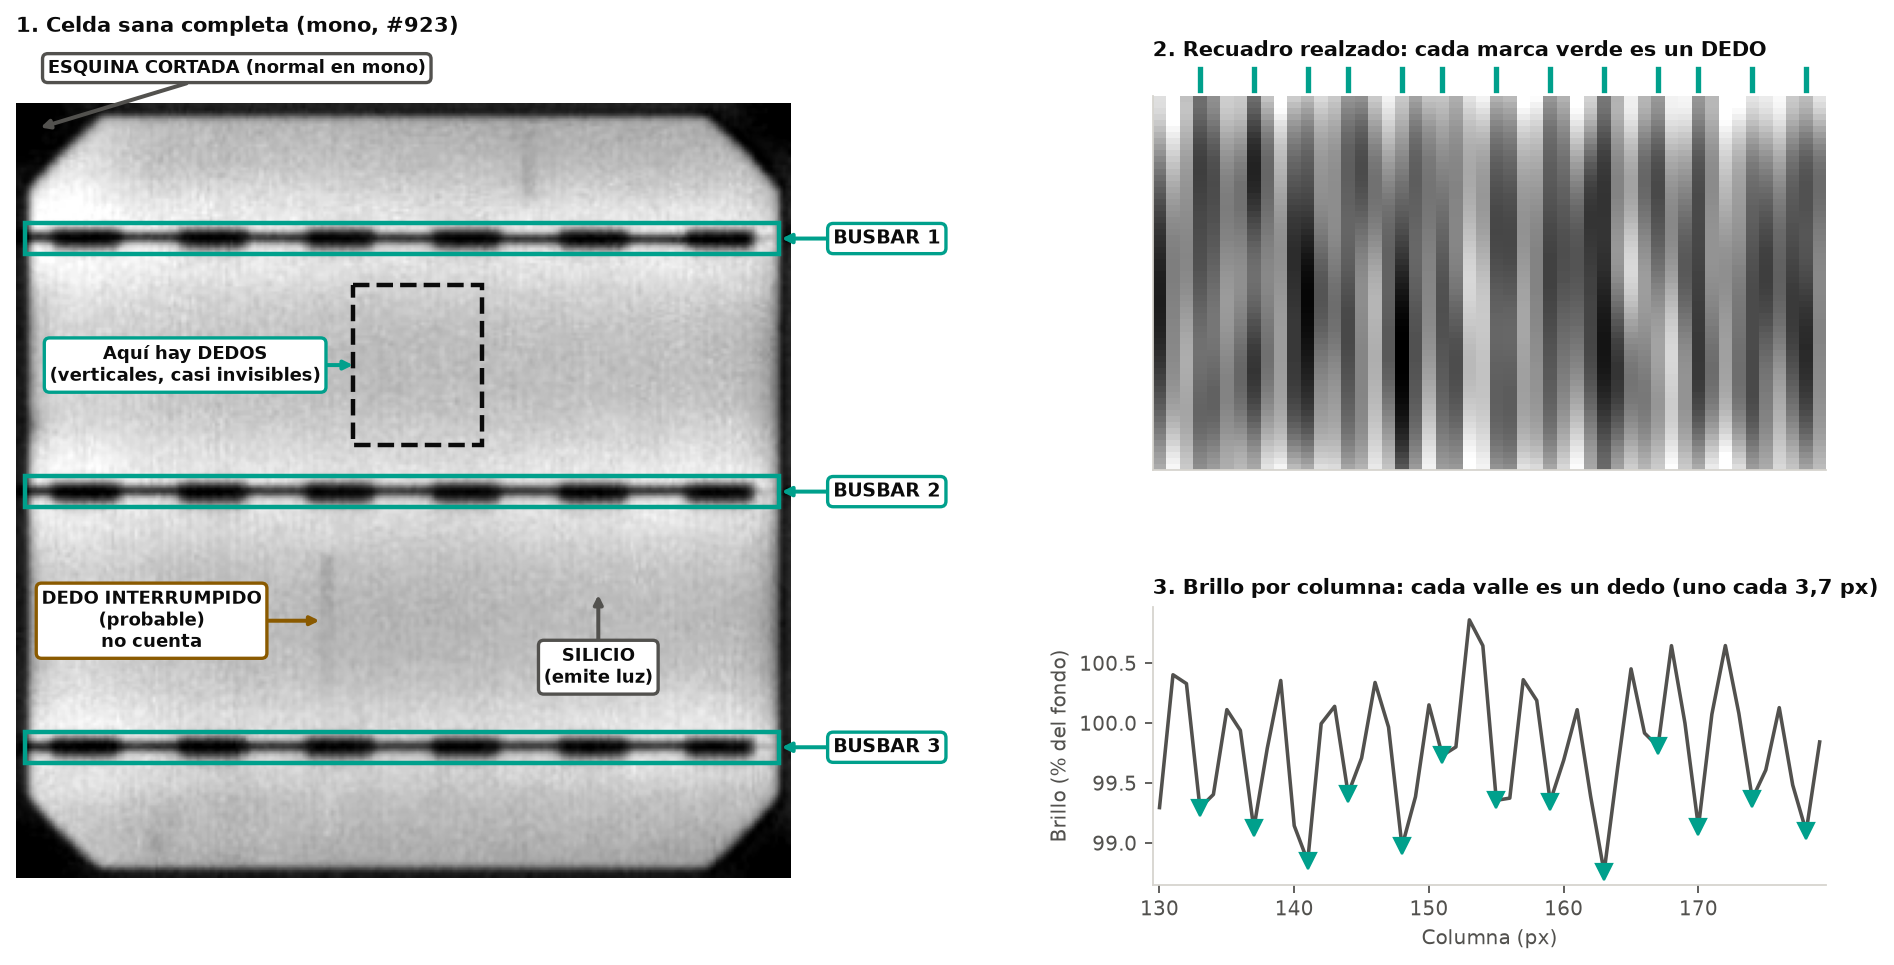
\includegraphics[width=0.6\textwidth]{b0a_anatomia_celda.png}
\caption{Qué se quita. Los \textbf{busbars} son las barras horizontales que reúnen la corriente. Los \textbf{dedos} son los hilos verticales que
la recogen del silicio; en esta celda solo se ven al realzar la imagen.}
\end{figure}

\paragraph{Detección v2.} Se calcula el sombrero negro vertical relativo de $I_n$ (alto 27 px): cuánto se hunde cada píxel respecto a lo que tiene arriba y
abajo. Una fila es candidata si la mediana a lo ancho supera 0,06, al menos el 60\,\% del ancho se hunde más de 0,03 y la banda mide como mucho
16 px. Una mancha más gruesa y la caída de brillo hacia el borde dan cero, y eran las dos fallas de la v1. Después se exige la geometría de la
rejilla: tres bandas separadas $\approx$98 px o dos separadas $\approx$143 px, centradas en la celda. Si de tres bandas falta una, tapada por una mancha, se infiere
(6 celdas). Los umbrales se ajustaron mirando los fallos en entrenamiento.

\paragraph{Referencia para medirla.} ELPV no anota los busbars. Leímos la rejilla en la imagen mediana de cada panel de entrenamiento y validación, donde las
manchas de cada celda se cancelan: 30 paneles tienen tres busbars, 6 tienen dos y uno no tiene ninguno. Una celda cuenta como correcta si coinciden el número y
todas las posiciones ($\pm$9 px).

\paragraph{A · Notch gaussiano (ec. 2).} $I_A=\mathcal F^{-1}\{H\,F\}$, con agujeros en $(0,\pm k v_0)$, $v_0=300/P$ y $P$ medido en cada celda. Usamos
$\sigma_n=1$, porque es lo más ancho que mantiene los agujeros separados ($\sigma_n\le v_0/2$, y $v_0=2{,}1$ con dos busbars), y $K=24$ armónicos. Se mide en
toda la celda (\textbf{A-global}) y solo en las filas de busbar (\textbf{A-filas}).

\paragraph{B · Cierre (ec. 3).} Elemento vertical de $h=21$ px, solo en las filas de busbar. Fue el de menor resto por tramos en el barrido de entrenamiento
(200 celdas sanas). Las bandas miden unos 8 px.

\paragraph{Dedos.} Cierre horizontal de $1\times3$, $1\times5$ y $1\times7$ sobre la salida de B. Se compara la respuesta del filtro de Sato antes y después, con los
parámetros de la línea base, como pide §4.3.

\paragraph{Grietas sintéticas (apoyo, no está en la tabla 3).} En 80 celdas sanas de validación se dibuja una línea oscura ($\sigma=1$ px, 70 px de largo, 20\,\% de
contraste) a distintos ángulos. Se mide qué fracción de ese contraste queda después de cada método.

\begin{figure}[H]
\centering
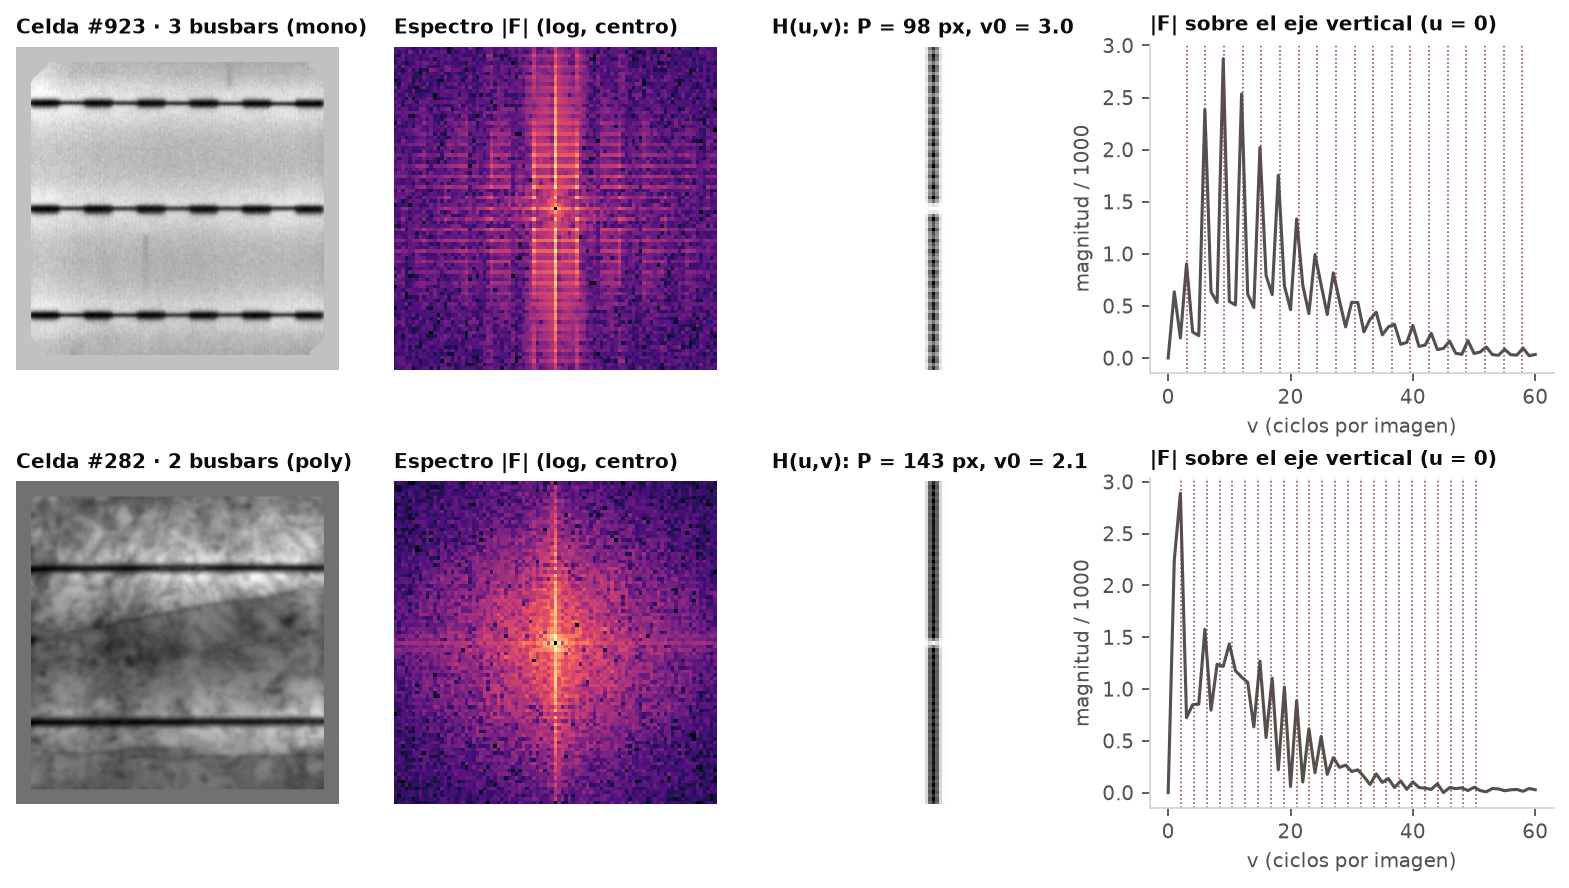
\includegraphics[width=0.56\textwidth]{b1_espectro_notch.png}
\caption{Espectro y filtro $H(u,v)$ en una celda de tres busbars y en una de dos. La rejilla deja picos en $kv_0$ (líneas punteadas) sobre el eje vertical. En la
punteada (\#923) hay además energía a los lados del eje, que los agujeros no alcanzan.}
\end{figure}

\section*{4 \quad Resultados}

\subsection*{4.1 \quad La detección nueva encuentra la rejilla}

\begin{figure}[H]
\centering
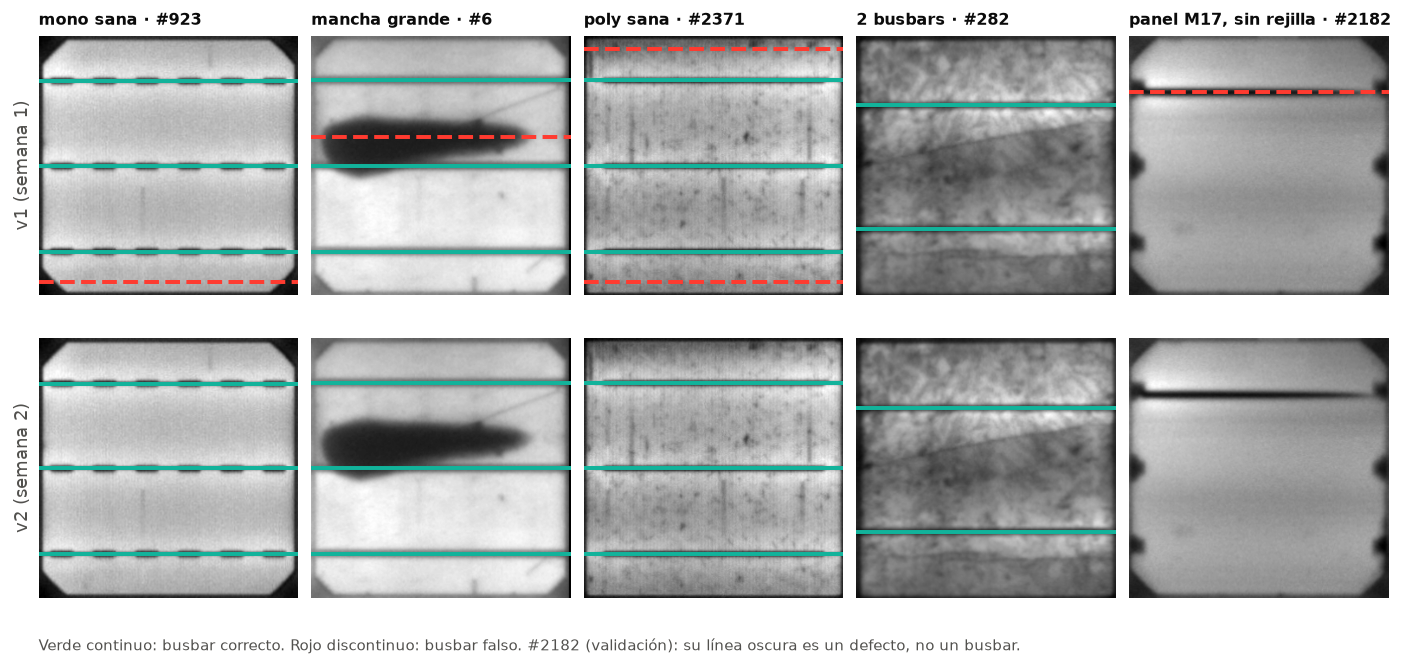
\includegraphics[width=0.66\textwidth]{b5_deteccion_v1_v2.png}
\caption{Busbars correctos (verde) y falsos (rojo). La v1 toma por busbar el borde oscuro, una mancha y el defecto horizontal de \#2182.}
\end{figure}

\begin{table}[H]
\centering\small
\begin{tabular}{@{}l r cc cc@{}}
\toprule
 & & \multicolumn{2}{c}{Rejilla exacta} & \multicolumn{2}{c}{Bandas falsas por celda} \\
\cmidrule(lr){3-4}\cmidrule(lr){5-6}
 & Celdas & v1 & v2 & v1 & v2 \\
\midrule
Entrenamiento & 1.790 & 13,7\,\% & \textbf{99,6\,\%} & 1,19 & \textbf{0} \\
Validación, mono & 192 & 16,1\,\% & \textbf{100\,\%} & 1,09 & \textbf{0} \\
Validación, poly & 240 & 8,3\,\% & \textbf{100\,\%} & 1,41 & \textbf{0} \\
\bottomrule
\end{tabular}
\caption{Detección de la rejilla. Los 7 fallos de la v2 son celdas de entrenamiento casi apagadas, todas defectuosas: no marca ninguna banda en ellas.}
\end{table}

\textbf{Hallazgo: el panel M17 no tiene busbars al frente.} Sus 72 celdas, todas mono y de validación, parecen de contacto trasero. Ningún panel de
entrenamiento es así. Son el 37,5\,\% de las mono de validación, así que las métricas de mono se reportarán con y sin M17.

\subsection*{4.2 \quad Criterios de la tabla 3 en validación}

\begin{figure}[H]
\centering
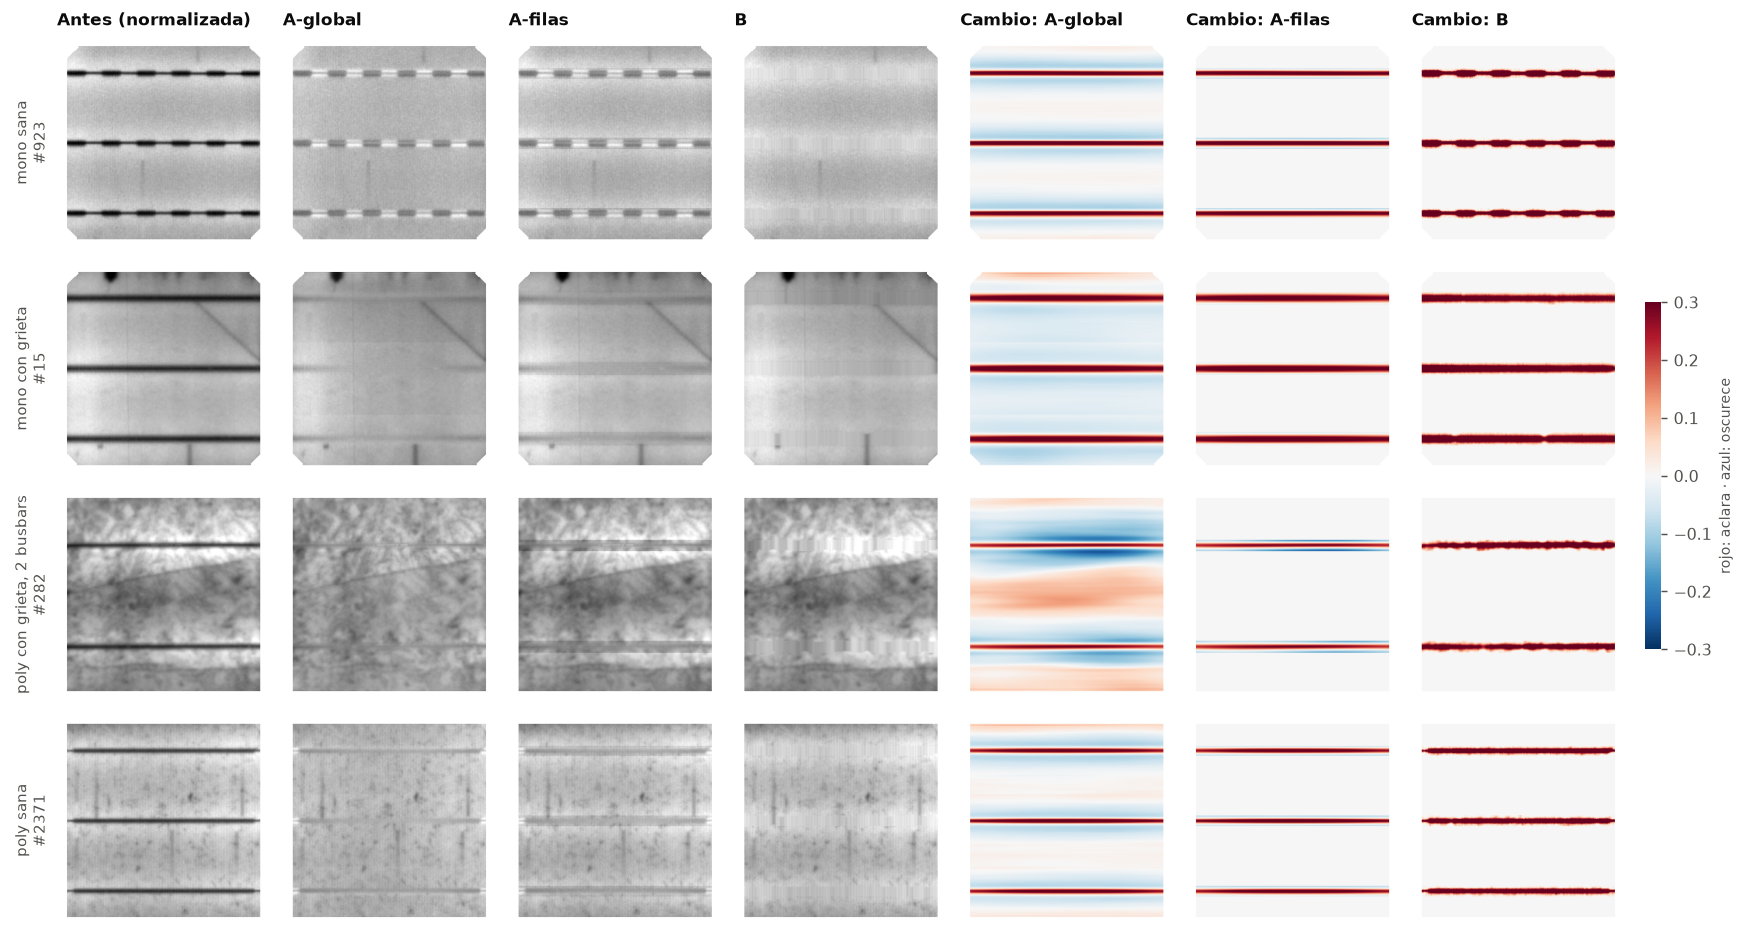
\includegraphics[width=0.74\textwidth]{b2_antes_despues.png}
\caption{Antes y después en cuatro celdas, y el cambio que introduce cada método.}
\end{figure}

\begin{table}[H]
\centering\small\setlength{\tabcolsep}{5pt}
\begin{tabular}{@{}l ccc ccc c r@{}}
\toprule
 & \multicolumn{3}{c}{1 · Resto del busbar} & \multicolumn{3}{c}{2 · Cambio fuera} & 4 · Tiempo & Falsa grieta \\
\cmidrule(lr){2-4}\cmidrule(lr){5-7}
 & todas & mono & poly & todas & mono & poly & ms/celda & mono / poly (px) \\
\midrule
Sin tocar & 40,3\,\% & 41,4\,\% & 39,7\,\% & 0 & 0 & 0 & – & 4.258 / 3.532 \\
A-global  & 5,9\,\%  & 6,1\,\%  & 5,9\,\%  & 3,4\,\% & 3,1\,\% & 3,5\,\% & 8,5 & 2.237 / 264 \\
A-filas   & 11,7\,\% & 11,6\,\% & 11,8\,\% & 0 & 0 & 0 & 9,5 & 3.178 / 164 \\
B         & \textbf{0,9\,\%} & \textbf{1,1\,\%} & \textbf{0,8\,\%} & 0 & 0 & 0 & \textbf{0,8} & 82 / 262 \\
\bottomrule
\end{tabular}
\caption{360 celdas de validación con rejilla (120 mono, 240 poly). Criterio 1: diferencia de brillo entre el busbar y sus filas vecinas. Criterio 2: cambio medio
fuera de las bandas, en \% del brillo sano; A-filas y B dan 0 por construcción. Falsa grieta (apoyo): mediana de píxeles que el filtro de Sato
marca en las celdas sanas.}
\end{table}

\begin{itemize}[leftmargin=14pt]
  \item \textbf{B limpia la banda casi por completo}, y además es unas diez veces más rápido (sin contar la detección, 2,1 ms, común a todos).
  \item \textbf{El notch deja la banda a medias} donde el busbar no es uniforme. En la rejilla punteada, la energía de los tramos gruesos cae fuera del eje
        vertical y ningún agujero la toca (celda \#923). Por eso en mono deja miles de píxeles de falsa grieta.
  \item \textbf{A-filas queda peor que A-global en el criterio 1}, porque el notch también baja el brillo alrededor del busbar y el parche ya no coincide con sus vecinas.
  \item \textbf{A-global altera el resto de la celda.} En poly aplana el brillo lento, que puede ser un defecto (\#282). En \#15 deja copias del borde: el \emph{ringing} que anticipó la propuesta.
  \item \textbf{Con dos busbars el notch también funciona}: resto del 6,2\,\%, frente a 5,9\,\% con tres.
\end{itemize}

\begin{figure}[H]
\centering
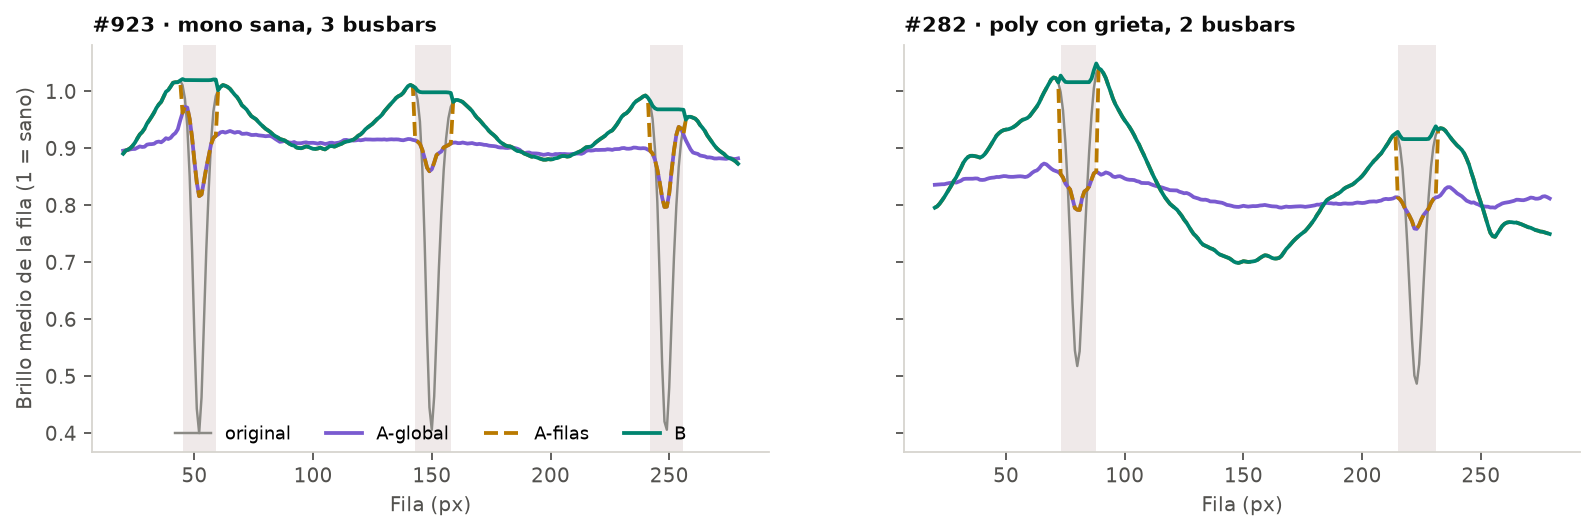
\includegraphics[width=0.62\textwidth]{b3_perfil_filas.png}
\caption{Brillo medio por fila antes y después. En gris claro, las filas de busbar.}
\end{figure}

\subsection*{4.3 \quad Cada método borra un tipo distinto de grieta}

\begin{figure}[H]
\centering
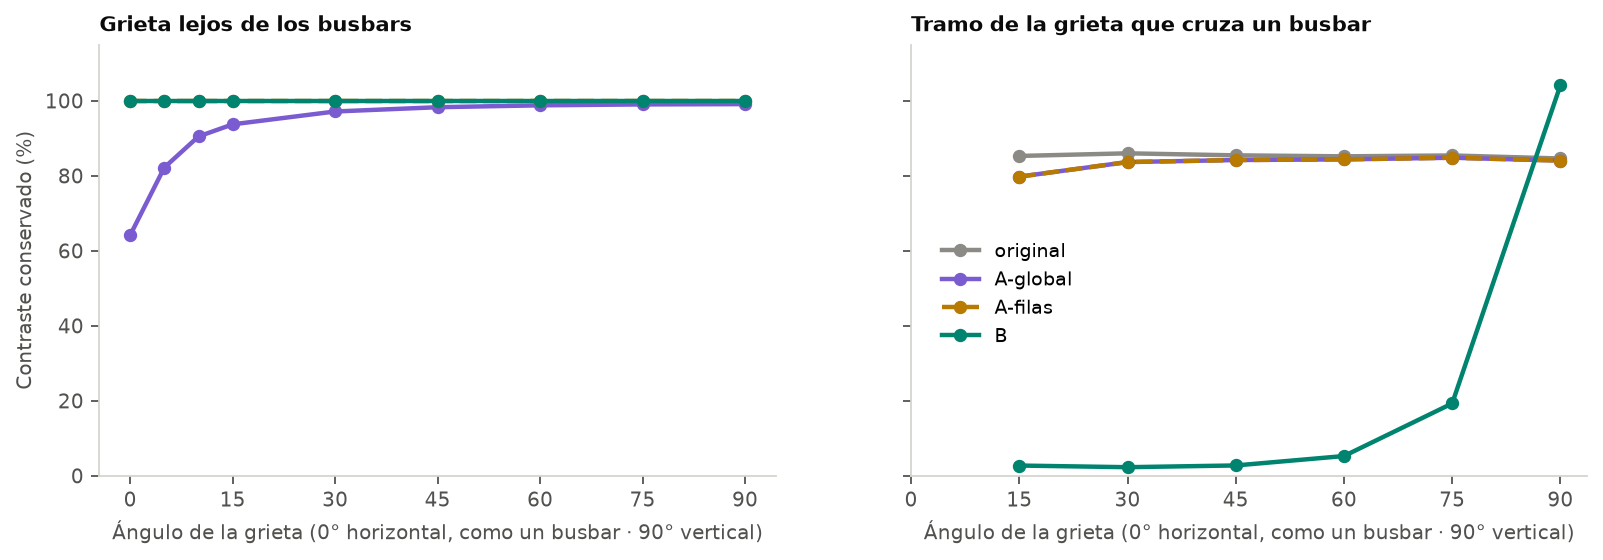
\includegraphics[width=0.66\textwidth]{b6_grietas_por_angulo.png}
\caption{Contraste que conserva una grieta sintética según su ángulo. Izquierda: A-filas y B coinciden en 100\,\%. Derecha: aun sin tocar la celda queda un 85\,\%, porque
bajo el busbar la grieta se ve menos.}
\end{figure}

\begin{itemize}[leftmargin=14pt]
  \item \textbf{A-global} le quita el 36\,\% del contraste a una grieta horizontal, porque su energía cae sobre el mismo eje que la rejilla. Con $\sigma_n=3$ se perdería
        el 82\,\%: es el costo de abrir más los agujeros para bajar el resto al 1,3\,\% (en entrenamiento).
  \item \textbf{B} borra el tramo de la grieta que pasa por la banda (3\,\% a 45°, 19\,\% a 75°). Solo respeta las verticales. La banda cubre unos 14 px por busbar.
  \item Es la primera razón concreta por la que el criterio 3 puede contradecir a los otros tres.
\end{itemize}

\subsection*{4.4 \quad Quitar los dedos no ayuda y debilita las grietas verticales}

\begin{figure}[H]
\centering
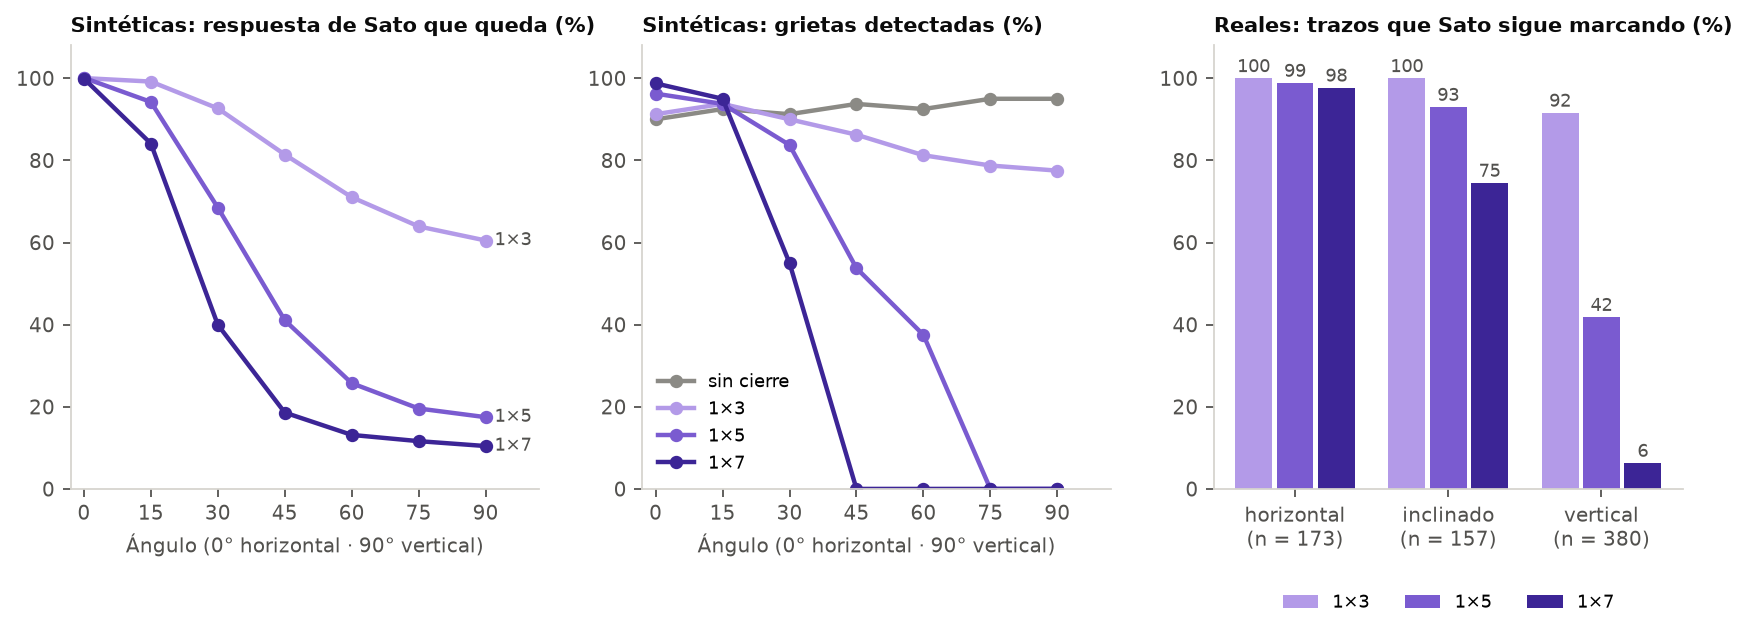
\includegraphics[width=0.8\textwidth]{b4b_sato_dedos.png}
\caption{Validación, sobre la salida de B. Izquierda y centro: grietas sintéticas de 60 px en 80 celdas sanas. Derecha: trazos reales que Sato marca sin cierre de dedos y
cuántos sigue marcando después.}
\end{figure}

\begin{table}[H]
\centering\footnotesize\setlength{\tabcolsep}{4.5pt}
\begin{tabular}{@{}l cc cc cc cc@{}}
\toprule
 & \multicolumn{2}{c}{Contraste de los dedos} & \multicolumn{2}{c}{Falsa grieta, sanas (px)} & \multicolumn{2}{c}{Sato, vertical sintética} & \multicolumn{2}{c}{Trazos verticales reales} \\
\cmidrule(lr){2-3}\cmidrule(lr){4-5}\cmidrule(lr){6-7}\cmidrule(lr){8-9}
 & mono & poly & mono & poly & respuesta & detectadas & respuesta & siguen \\
\midrule
Sin quitar   & 0,08\,\% & 0,16\,\% & 89  & 523 & 100\,\% & 95\,\% & 100\,\% & 100\,\% \\
$1\times3$   & 0,04\,\% & 0,11\,\% & 119 & 544 & 60\,\%  & 78\,\% & 91\,\%  & 92\,\% \\
$1\times5$   & 0,05\,\% & 0,09\,\% & 123 & 458 & 17\,\%  & 0\,\%  & 62\,\%  & 42\,\% \\
$1\times7$   & 0,03\,\% & 0,08\,\% & 100 & 463 & 10\,\%  & 0\,\%  & 32\,\%  & 6\,\% \\
\bottomrule
\end{tabular}
\caption{Validación, 360 celdas con rejilla. Contraste: mediana de la amplitud del patrón periódico. Falsa grieta: media por celda sana (40 mono, 138 poly).
Trazos reales: 380 de más de 25 px y a menos de 30° de la vertical; mediana de la respuesta y \% que Sato sigue marcando. Se excluyen M17 y el borde lateral de la máscara.}
\end{table}

\begin{figure}[H]
\centering
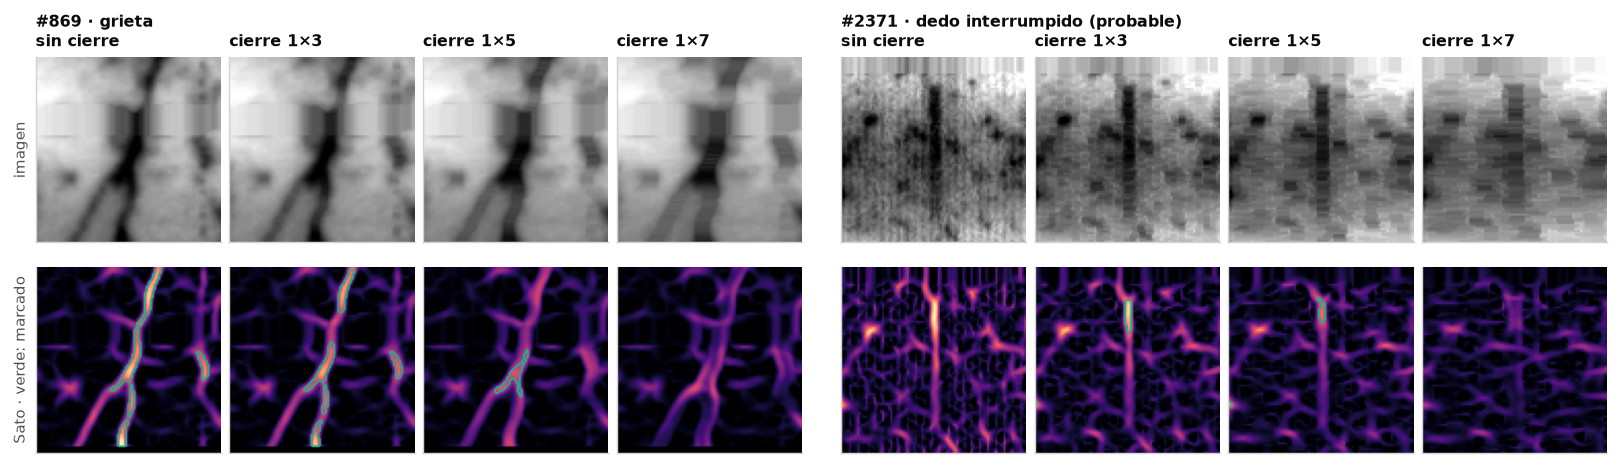
\includegraphics[width=0.92\textwidth]{b4_grietas_verticales.png}
\caption{Antes y después de quitar los dedos en dos celdas de entrenamiento. Arriba, la imagen; abajo, la respuesta de Sato, con lo marcado en verde. Con $1\times7$ ya no se marca la grieta.}
\end{figure}

\begin{itemize}[leftmargin=14pt]
  \item \textbf{No hay beneficio que compense.} Los dedos modulan el brillo muy poco. El cierre no baja las falsas grietas en mono (89 a 119 px con $1\times3$), y en poly solo
        las baja un 12\,\% con $1\times5$.
  \item \textbf{$1\times5$ y $1\times7$ quedan descartados.} Ninguna grieta vertical fina sintética se detecta después, y de los trazos reales sobrevive menos de la mitad.
  \item \textbf{$1\times3$ es más suave de lo que sugieren las sintéticas.} En los trazos reales, que suelen ser más gruesos, la respuesta baja un 9\,\%. En grietas finas baja un 40\,\%;
        en mono se siguen detectando todas, pero en poly la detección cae del 90\,\% al 55\,\%.
  \item \textbf{El cierre no distingue grietas de dedos interrumpidos.} Los trazos verticales pierden lo mismo en celdas sanas que en defectuosas (siguen el 91\,\% en ambas con
        $1\times3$). En las sanas lo más probable es que sean dedos interrumpidos, que ELPV no cuenta como defecto.
  \item \textbf{Límite:} los trazos reales son los que Sato ya marcaba sin cierre, y ELPV no dice cuáles son grietas.
\end{itemize}

\section*{5 \quad Decisiones y cambios respecto a la propuesta}

\begin{table}[H]
\centering\small
\begin{tabularx}{\textwidth}{@{}>{\raggedright}p{4.4cm} X@{}}
\toprule
Decisión & Por qué \\
\midrule
Detección v2 en lugar de la v1 & La v1 acierta la rejilla en el 12\,\% de validación. La línea base del Avance 1 no se toca: \texttt{src/preproc.py} sigue igual. \\
\textbf{Propuesta de cambio:} no quitar los dedos (§4.3) & Debilita las grietas verticales y no reduce las falsas en mono. La CNN se entrenará también con dedos quitados ($1\times3$) para confirmarlo. \\
Mono con y sin M17 & Sin busbars, M17 no distingue entre A y B, y pesa el 37,5\,\% de las mono de validación. \\
Grietas sintéticas como apoyo & Los criterios 1 y 2 no ven lo que B borra dentro de la banda. No cambian la regla: decide el criterio 3. \\
M17 fuera de las medidas de dedos y trazos & Sus pestañas laterales dan 328 trazos verticales falsos en validación, y no tiene dedos al frente. \\
\bottomrule
\end{tabularx}
\end{table}

\textbf{Sin cambios en el alcance.} La partición sigue congelada y el conjunto de prueba no se ha usado.

\section*{6 \quad Problemas, límites y riesgos}

\begin{itemize}[leftmargin=14pt]
  \item \textbf{La referencia de la detección es nuestra.} Es una lectura por panel, no una anotación externa. Para hacerla vimos las imágenes medianas de los paneles de
        validación y algunas celdas de M17, así que el 100\,\% de validación no es del todo a ciegas. Los umbrales se ajustaron con los errores de entrenamiento, pero la
        regla de exigir al menos dos bandas se escribió después de ver \#2182.
  \item \textbf{Las grietas sintéticas son una simplificación}: rectas, del mismo grosor y contraste. Sirven para comparar métodos, no para predecir aciertos.
  \item \textbf{Los rótulos de defectos} de las figuras \texttt{b0} y de la página son lectura visual; los dedos interrumpidos figuran como probables.
  \item \textbf{Cambio de dominio por M17.} La CNN no verá ninguna celda sin rejilla al entrenar. Puede pasar también en la prueba, que no hemos mirado.
  \item \textbf{Granos de poly.} Siguen marcando falsas grietas aun sin rejilla (262 px). Es la tarea principal de la semana 3.
\end{itemize}

\section*{7 \quad Plan de la semana 3: mapas y CNN}

\begin{enumerate}[leftmargin=16pt]
  \item Mapa de grietas con Sato y, en poly, Gabor y filtrado por orientación y longitud. Mapa de zonas apagadas.
  \item CNN de 3 canales a $128\times128$, con tres semillas: con \textbf{A}, con \textbf{B} y con la imagen original. Además, B con y sin dedos.
  \item \textbf{Elegir con el criterio 3}, reportar mono con y sin M17, y congelar el sistema.
\end{enumerate}

\vspace{4pt}
\begin{ojo}{Reproducir.}
Desde la raíz del repo, con el entorno de \texttt{requirements.txt}: \texttt{scripts/06\_figuras\_anatomia.py}, \texttt{scripts/07\_comparar\_busbars.py} ($\sim$4 min),
\texttt{scripts/08\_exportar\_web.py} y \texttt{scripts/09\_grietas\_verticales.py}. Las cifras quedan en \texttt{reports/metricas/semana2\_*.json}. La página
\texttt{entregas/avance\_2/web/laboratorio\_busbars.html} se abre con doble clic y repite el notch y el cierre en vivo. Los tiempos dependen del equipo (un hilo, mediana de 120 celdas).
\end{ojo}

{\small
\sloppy\textbf{Referencias.}
[1] S. Deitsch \emph{et al.}, «Automatic classification of defective photovoltaic module cells in electroluminescence images», \emph{Solar Energy}, vol. 185,
pp. 455–468, 2019. ·
[2] ZAE Bayern, «elpv-dataset», \url{github.com/zae-bayern/elpv-dataset}. Imágenes con licencia CC BY-NC-SA 4.0.
}

\end{document}
